\subsection{Principal Minors and Inertia}

\begin{definition} \label{def:principal-and-leading-principal-minors} \hlt{Principal and Leading Principal Minors}\\
For $A\in\operatorname{Mat}(n,n,\mathbb{C})$, a \hlt{principal minor} is the determinant of a principal submatrix of $A$.\\
A \hlt{leading principal minor} is the determinant of the leading $k\times k$ principal submatrix for some $k=1,\ldots,n$.
\end{definition}

\begin{corollary} \label{cor:positive-semidefinite-principal-block-column-inclusion} \hlt{Principal Blocks and Column Inclusion}\\
Let $A\in\operatorname{Mat}(n,n,\mathbb{F})$ be PSD, where $\mathbb{F}\in\{\mathbb{R},\mathbb{C}\}$, and partition $A=
\begin{bmatrix}
A_{11} & A_{12}\\
A_{12}^* & A_{22}
\end{bmatrix}$, $A_{11}\in\operatorname{Mat}(k,k,\mathbb{F})$.\\
Then $A_{11}\succeq0$, $\operatorname{col}(A_{12})\subseteq\operatorname{col}(A_{11})$, and $\operatorname{rank}(A_{12})\leq\operatorname{rank}(A_{11})$. If $A\succ0$, then $A_{11}\succ0$.
\begin{proof}
Write $A=B^*B$ and partition $B=[B_1\ B_2]$ conformally. Then $A_{11}=B_1^*B_1$ and $A_{12}=B_1^*B_2$.\\
Hence $A_{11}\succeq0$ and $\operatorname{col}(A_{12})=\operatorname{col}(B_1^*B_2)\subseteq\operatorname{col}(B_1^*)=\operatorname{col}(B_1^*B_1)=\operatorname{col}(A_{11})$, equality $\operatorname{col}(B_1^*)=\operatorname{col}(B_1^*B_1)$ follows from Theorem \ref{thm:gram-factor-kernel-rank-column-data}. The rank inequality follows by taking dimensions\\
If $A\succ0$ and $\mathbf{x}\neq0$ in $\mathbb{F}^k$, then $\mathbf{x}^*A_{11}\mathbf{x}=
\begin{bmatrix}\mathbf{x}\\0\end{bmatrix}^*
A
\begin{bmatrix}\mathbf{x}\\0\end{bmatrix}>0$, so $A_{11}\succ0$.\\
\hlt{Structural Commentary}: In a positive block matrix, cross-block columns lie in principal block's column space.\\
\hlt{Key Insight}: Factor first; then column inclusion is immediate from $A_{12}=B_1^*B_2$.
\end{proof}
\end{corollary}

\begin{figure}[H]
  \centering
  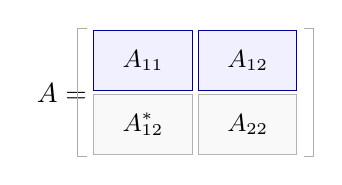
\begin{tikzpicture}[
  every node/.style={font=\small},
  block/.style={draw=gray!60, fill=gray!5, minimum width=1.25cm, minimum height=0.76cm, align=center},
  focus/.style={draw=blue!60!black, fill=blue!6}
]
  \node[block, focus] (a11) at (0,0) {$A_{11}$};
  \node[block, focus] (a12) at (1.33,0) {$A_{12}$};
  \node[block] (a21) at (0,-0.81) {$A_{12}^*$};
  \node[block] (a22) at (1.33,-0.81) {$A_{22}$};

  \node[font=\normalsize] at (-1.03,-0.41) {$A=$};
  \draw[gray!65] (-0.71,0.41) -- (-0.83,0.41) -- (-0.83,-1.22) -- (-0.71,-1.22);
  \draw[gray!65] (2.04,0.41) -- (2.16,0.41) -- (2.16,-1.22) -- (2.04,-1.22);
\end{tikzpicture}

  \caption{For $A\succeq0$, factorisation forces $\operatorname{col}(A_{12})\subseteq\operatorname{col}(A_{11})$.}
  \label{fig:principal-block-column-inclusion}
\end{figure}

\begin{theorem} \label{thm:sylvester-positive-definite-criterion-leading-minors} \hlt{Sylvester's Criterion}\\
A Hermitian matrix $A\in\operatorname{Mat}(n,n,\mathbb{C})$ is positive definite if and only if all leading principal minors are positive.
\begin{proof}
\begin{enumerate}[label=\roman*.]
\setlength{\itemsep}{0pt}
\item[$(\Rightarrow)$] If $A\succ0$, then each leading principal submatrix is positive definite by Corollary \ref{cor:positive-semidefinite-principal-block-column-inclusion}. Its eigenvalues are positive, so its determinant is positive.
\item[$(\Leftarrow)$] Induct on $n$. If $n=1$, the single leading principal minor is the only diagonal entry, so positivity of that minor is exactly positive definiteness. Assume $n\geq2$ and write $A=
\begin{bmatrix}
B & \mathbf{y}\\
\mathbf{y}^* & a
\end{bmatrix}$, $B\in\operatorname{Mat}(n-1,n-1,\mathbb{C})$\\
The leading principal minors of $B$ are positive, so $B\succ0$.\\
Since $\det(B)>0$ and $\det(A)>0$, Proposition \ref{prop:schur-complement-determinant-formula} gives $a-\mathbf{y}^*B^{-1}\mathbf{y}=\frac{\det(A)}{\det(B)}>0$.\\
For $\mathbf{u}\in\mathbb{C}^{n-1}$ and $t\in\mathbb{C}$, $\begin{bmatrix}\mathbf{u}\\ t\end{bmatrix}^*
A
\begin{bmatrix}\mathbf{u}\\ t\end{bmatrix} =(\mathbf{u}+B^{-1}\mathbf{y}t)^*B(\mathbf{u}+B^{-1}\mathbf{y}t) +\left(a-\mathbf{y}^*B^{-1}\mathbf{y}\right)\abs{t}^2$.\\
First term is nonnegative as $B\succ0$, and second coefficient is positive. If displayed vector is nonzero, then either $t\neq0$ and second term is positive, or $t=0$ and then $\mathbf{u}\neq0$, making first term positive. Thus $A\succ0$.
\end{enumerate}
\hlt{Structural Commentary}: Leading minors make each leading block positive and final Schur complement positive.\\
\hlt{Key Insight}: Complete the square with the leading block.
\end{proof}
\end{theorem}

\begin{method} \label{meth:two-by-two-quadratic-form-test} \hlt{$2\times2$ Quadratic Form Test}\\
Let $A=\begin{bmatrix}a&b\\ b&c\end{bmatrix}$ be real symmetric, $\Delta=ac-b^2$, and $q(x,y)=\begin{bmatrix}x&y\end{bmatrix}A\begin{bmatrix}x\\y\end{bmatrix}=ax^2+2bxy+cy^2$.\\
For $a\neq0$, $q(x,y)=a\left(x+\frac{b}{a}y\right)^2+\frac{\Delta}{a}y^2$.\\
If $a=0$, swap variables when $c\neq0$; if $a=c=0$, use $q=2bxy$. Thus:
\begin{enumerate}[label=(\roman*)]
\setlength{\itemsep}{0pt}
\item $q\succ0$ if and only if $a>0$ and $\Delta>0$;
\item $q\prec0$ if and only if $a<0$ and $\Delta>0$;
\item $q$ is indefinite if and only if $\Delta<0$;
\item if $\Delta=0$, then $q\succeq0$ iff $a,c\geq0$, and $q\preceq0$ iff $a,c\leq0$.
\end{enumerate}
This is the $2\times2$ form of Sylvester's criterion and inertia.\\
\hlt{Structural Commentary}: Completing the square is the $2\times2$ shadow of the $LDL^*$ and Schur-complement tests.\\
\hlt{Key Insight}: $\Delta$ and the leading sign classify the form.
\end{method}

\begin{theorem} \label{thm:real-quadratic-form-principal-axes} \hlt{Principal Axes for Real Quadratic Forms}\\
Let $A\in\operatorname{Mat}(n,n,\mathbb{R})$ be symmetric. Then:
\begin{enumerate}[label=(\roman*)]
\setlength{\itemsep}{0pt}
\item there are a real orthogonal $Q$ and real $\lambda_1,\ldots,\lambda_n$ such that, with $\mathbf{y}=Q^t\mathbf{x}$, $\mathbf{x}^tA\mathbf{x}=\sum\limits_{j=1}^{n}\lambda_jy_j^2$.
\item $A\succeq0$ if and only if every $\lambda_j\geq0$;
\item $A\succ0$ if and only if every $\lambda_j>0$;
\item $A$ is indefinite if and only if some $\lambda_j>0$ and some $\lambda_k<0$.
\end{enumerate}
\begin{proof}
\begin{enumerate}[label=(\roman*)]
\setlength{\itemsep}{0pt}
\item By the real spectral theorem, write $A=Q\operatorname{diag}(\lambda_1,\ldots,\lambda_n)Q^t$.\\
Then $\mathbf{x}^tA\mathbf{x} =\mathbf{x}^tQ\operatorname{diag}(\lambda_j)Q^t\mathbf{x} =\mathbf{y}^t\operatorname{diag}(\lambda_j)\mathbf{y} =\sum\limits_{j=1}^{n}\lambda_jy_j^2$.
\item The displayed sum is nonnegative for all $\mathbf{y}$ exactly when each coefficient $\lambda_j$ is nonnegative.
\item The displayed sum is positive for all nonzero $\mathbf{y}$ exactly when each coefficient $\lambda_j$ is positive.
\item The diagonal form takes both signs exactly when its coefficients include both signs.
\end{enumerate}
\hlt{Structural Commentary}: Principal axes turn the form into signed squares.\\
\hlt{Key Insight}: Eigenvalue signs classify the quadratic form.
\end{proof}
\end{theorem}

\begin{method} \label{meth:quadratic-form-principal-axes} \hlt{Quadratic Form Principal-Axes Method}\\
To analyse a real quadratic form:
\begin{enumerate}[label=(\roman*)]
\setlength{\itemsep}{0pt}
\item write it as $\mathbf{x}^tA\mathbf{x}$ with $A=A^t$; split each cross coefficient equally between $a_{ij}$ and $a_{ji}$;
\item diagonalise $A=Q\Lambda Q^t$;
\item change variables by $\mathbf{y}=Q^t\mathbf{x}$;
\item classify the form from the signs of the eigenvalues in $\Lambda$.
\end{enumerate}
\end{method}

\begin{figure}[H]
  \centering
  \begin{tikzpicture}[
  >=Stealth,
  scale=0.95,
  axis/.style={->, gray!65, line width=0.65pt},
  paxis/.style={->, blue!70!black, line width=0.95pt},
  curve/.style={draw=teal!70!black, line width=0.9pt},
  every node/.style={font=\small}
]
  \draw[axis] (-2.2,0) -- (2.45,0) node[right] {$x_1$};
  \draw[axis] (0,-1.65) -- (0,1.9) node[above] {$x_2$};
  \draw[curve, rotate=28] (0,0) ellipse (1.65 and 0.72);

  \draw[paxis] (0,0) -- (1.28,0.68) node[pos=0.86, above right] {$\mathbf{q}_1$};
  \draw[paxis] (0,0) -- (-0.38,0.72) node[pos=0.86, above left] {$\mathbf{q}_2$};

  \node[align=center] at (5.15,0.95) {$\mathbf{y}=Q^t\mathbf{x}$};
  \draw[->, line width=0.8pt, gray!65] (2.55,0.25) -- (3.85,0.25);

  \begin{scope}[shift={(6.15,0)}]
    \draw[axis] (-1.85,0) -- (2.0,0) node[right] {$y_1$};
    \draw[axis] (0,-1.45) -- (0,1.6) node[above] {$y_2$};
    \draw[curve] (0,0) ellipse (1.45 and 0.65);
  \end{scope}

  \node[align=center, text=teal!60!black] at (6.15,-1.65) {$\lambda_1y_1^2+\lambda_2y_2^2$};
\end{tikzpicture}

  \caption{Orthogonal coordinates reveal the principal axes of a quadratic form.}
  \label{fig:quadratic-form-principal-axes}
\end{figure}

\begin{definition} \label{def:star-congruence-and-hermitian-inertia} \hlt{$*$-Congruence and Hermitian Inertia}\\
Two matrices $A,B\in\operatorname{Mat}(n,n,\mathbb{C})$ are \hlt{$*$-congruent} if $A=SBS^*$ for some invertible $S\in\operatorname{Mat}(n,n,\mathbb{C})$.\\
For Hermitian $A$, its \hlt{inertia} is $\operatorname{in}(A)=(n_+(A),n_-(A),n_0(A))$, where these are the numbers of positive, negative, and zero eigenvalues of $A$, counted with multiplicity.
\end{definition}

\begin{lemma} \label{lem:positive-subspace-dimension-inertia} \hlt{Positive Subspaces and Inertia}\\
Let $A\in\operatorname{Mat}(n,n,\mathbb{C})$ be Hermitian. The maximal dimensions of subspaces on which $\mathbf{x}^*A\mathbf{x}$ is positive or negative for every nonzero $\mathbf{x}$ are $n_+(A)$ and $n_-(A)$, respectively.
\begin{proof}
Let $P_+$, $P_{\leq0}$ be positive, nonpositive spectral subspaces. Then $\dim P_+=n_+(A)$, $P_+$ is positive for $A$.\\
If $\dim\mathcal{U}>n_+(A)$, then $\dim\mathcal{U}+\dim P_{\leq0}>n_+(A)+n_-(A)+n_0(A)=n$, so $\mathcal{U}\cap P_{\leq0}$ contains a nonzero vector.\\
On this vector quadratic form is nonpositive, so $\mathcal{U}$ cannot be positive. Apply this to $-A$ for negative case.\\
\hlt{Structural Commentary}: The positive spectral subspace is maximal; the nonpositive part blocks enlargement.\\
\hlt{Key Insight}: Inertia counts maximal sign-definite dimensions.
\end{proof}
\end{lemma}

\begin{theorem} \label{thm:sylvester-inertia-theorem-hermitian} \hlt{Sylvester's Inertia Theorem}\\
Hermitian matrices $A,B$ of the same size are $*$-congruent if and only if $n_+(A)=n_+(B)$ and $n_-(A)=n_-(B)$.
\begin{proof}
\begin{enumerate}[label=\roman*.]
\setlength{\itemsep}{0pt}
\item[$(\Rightarrow)$] Suppose $A=SBS^*$ with $S$ invertible. Then $\mathbf{x}^*A\mathbf{x}=(S^*\mathbf{x})^*B(S^*\mathbf{x})$.\\
Thus $S^*$ transports positive and negative subspaces, so Lemma \ref{lem:positive-subspace-dimension-inertia} gives $n_\pm(A)=n_\pm(B)$.
\item[$(\Leftarrow)$] Let the common inertia be $(p,q,r)$ and set $D=I_p\oplus(-I_q)\oplus0_r$.\\
By the spectral theorem, each of $A$ and $B$ is $*$-congruent to $D$, hence they are $*$-congruent to each other.
\end{enumerate}
\hlt{Structural Commentary}: $*$-congruence is a coordinate change for Hermitian quadratic forms.\\
\hlt{Key Insight}: Spectral decomposition reduces the form to signed squares and zero directions.
\end{proof}
\end{theorem}

\begin{figure}[H]
  \centering
  \begin{tikzpicture}[
  >=Stealth,
  scale=0.92,
  axis/.style={->, gray!65, line width=0.65pt},
  posregion/.style={draw=blue!70!black, fill=blue!8, line width=0.9pt},
  negregion/.style={draw=red!70!black, fill=red!8, line width=0.9pt},
  zeroregion/.style={draw=gray!70, line width=0.9pt},
  lab/.style={font=\small, align=center},
  tiny/.style={font=\scriptsize, align=center}
]
  \begin{scope}
    \draw[axis] (-1.8,0) -- (1.95,0);
    \draw[axis] (0,-1.55) -- (0,1.75);
    \draw[posregion, rotate=22] (0,0) ellipse (1.45 and 0.55);
    \draw[negregion, rotate=-28] (0,0) ellipse (0.52 and 1.15);
    \draw[zeroregion] (-1.1,-1.1) -- (1.1,1.1);
    \node[lab] at (0,-2.0) {$\mathbf{x}^*A\mathbf{x}$};
  \end{scope}

  \draw[->, line width=0.9pt, gray!70] (2.35,0) -- (3.75,0)
    node[midway, above, lab] {$*$-congruence};

  \begin{scope}[shift={(5.45,0)}]
    \draw[axis] (-1.7,0) -- (1.9,0);
    \draw[axis] (0,-1.55) -- (0,1.75);
    \draw[blue!70!black, line width=1.25pt, ->] (0,0) -- (1.35,0) node[right, tiny] {$+1$};
    \draw[red!70!black, line width=1.25pt, ->] (0,0) -- (0,-1.2) node[below, tiny] {$-1$};
    \draw[gray!65, line width=1.25pt] (-1.2,1.0) -- (1.2,1.0) node[right, tiny] {$0$};
    \node[lab] at (0,-2.0) {$I_p\oplus(-I_q)\oplus0_r$};
  \end{scope}
\end{tikzpicture}

  \caption{$*$-congruence reduces a Hermitian form to signed coordinate axes.}
  \label{fig:sylvester-inertia-congruence}
\end{figure}
